\documentclass[a4paper,twoside,12pt]{book}
\usepackage[utf8]{inputenc}
\usepackage{natbib}
\usepackage{graphicx}
\usepackage[a4paper, left=37mm, right=27mm, top=39mm, bottom=39mm, headsep=12mm, footskip=15mm]{geometry}
\setlength{\headheight}{15pt}
\usepackage{fancyhdr}
\usepackage{fontenc}
\usepackage{float}
\usepackage{rotating}
\usepackage{hyperref}
\usepackage{afterpage}
\usepackage{mathtools}
\usepackage{amsmath}
\usepackage{tabu}
\usepackage{listings}
\usepackage{subcaption}
\usepackage{emptypage}
\usepackage{bookmark}
\usepackage{xfrac}
\usepackage{epsfig}

\pagestyle{fancy}
\renewcommand{\chaptermark}[1]{\markboth{#1}{}}
\renewcommand{\sectionmark}[1]{\markright{\thesection\ #1}}
\fancyhf{} \fancyhead[LE,RO]{\bfseries\thepage}
\fancyhead[LO]{\bfseries\rightmark}
\fancyhead[RE]{\bfseries\leftmark}
\renewcommand{\headrulewidth}{0.5pt}
\renewcommand{\footrulewidth}{0pt}
\fancypagestyle{plain}{
	\fancyhead{}
	\renewcommand{\headrulewidth}{0pt}}

%%%%%%%%%% General thesis informations go here! (TITLE, AUTHOR-NAME, KEYWORD-1, KEYWORD-2,...
\hypersetup{
    pdfauthor  = {AUTHOR-NAME},    		    % author
    pdftitle   = {TITLE},    				% title
 	pdfsubject = {Master's Degree Thesis},  % subject of the document
 	pdfkeywords= {KEYWORD-1, KEYWORD-2}      % list of keywords
}

%%%%%%%%%%%%%%%%%%%%%%%%%%%%%% BEGIN OF THE DOCUMENT
\begin{document}

\pagestyle{fancy}
\renewcommand{\chaptermark}[1]{\markboth{#1}{}}
\renewcommand{\sectionmark}[1]{\markright{\thesection\ #1}}
\fancyhf{} \fancyhead[LE,RO]{\bfseries\thepage}
\fancyhead[LO]{\bfseries\rightmark}
\fancyhead[RE]{\bfseries\leftmark}
\renewcommand{\headrulewidth}{0.5pt}
\renewcommand{\footrulewidth}{0pt}
\fancypagestyle{plain}{
	\fancyhead{}
	\renewcommand{\headrulewidth}{0pt}}

%%%%%%%%%%%%%%%%%%%%%%%%%%%%%% Title page	
\pagenumbering{gobble}
\newgeometry{margin=3cm}
\begin{titlepage}

\begin{center}
\Large\textbf{{\textsc{POLITECNICO DI MILANO}}}\\
\Large{Scuola di Ingegneria Industriale e dell'Informazione}\\
\large{Corso di Laurea Magistrale in Ingegneria Spaziale}\\
\large{Dipartimento di Scienze e Tecnologie Aerospaziali (DAER)}
\par\end{center}

\vspace{0.5cm}

\begin{center}
\begin{figure}[h]
\centering{}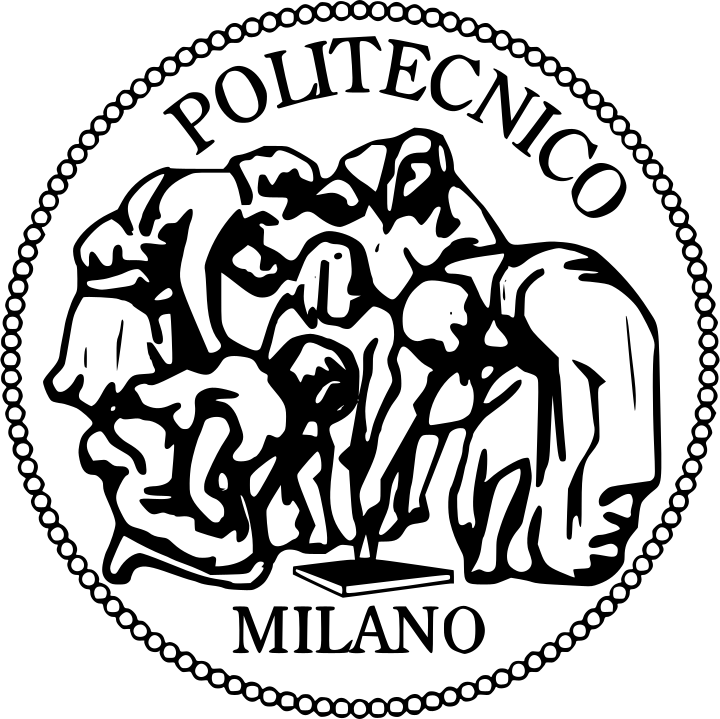
\includegraphics[width=0.3\textwidth]{title-page/logo-polimi}
\end{figure}
\vspace{0.5cm}
\par\end{center}

\begin{center}
\textbf{\LARGE{Analysis of a Vision-Based pose initialization algorithm for non-cooperative spacecraft on synthetic imagery}}\vspace{0.5cm}
\vspace{0.2cm}
\par\end{center}

\begin{center}
\textbf{D-Orbit}\\
\textit{in collaboration with}\\
\textbf{Space Missions Engineering Lab}
\end{center}\vspace{1.5cm}

\begin{flushleft}
\begin{tabular}{ll}
Relatore:  & Prof. Paolo LUNGHI\tabularnewline
Correlatore: & Dott. Ing. Aureliano RIVOLTA\tabularnewline
\end{tabular}\vspace{1.8cm}
\par\end{flushleft}

\begin{flushright}
\begin{tabular}{ll}
Tesi di laurea di: & \tabularnewline
Francescodario CUZZOCREA & Matr. 885016\tabularnewline
\end{tabular}\vspace{1.5cm}
\par\end{flushright}

\begin{center}
{\large{}Anno Accademico 2019-2020}{\large\par}
\par\end{center}

\end{titlepage}

\restoregeometry
\cleardoublepage{}

%%%%%%%%%%%%%%%%%%%%%%%%%%%%%% Dedication
\begin{flushright}
\emph{To someone very special\ldots{}
}
\par
\end{flushright}
\cleardoublepage{}

%%%%%%%%%%%%%%%%%%%%%%%%%%%%%% Acnowledgment
\pagenumbering{Roman}
\chapter*{Acknowledgments}
\addcontentsline{toc}{chapter}{Acknowledgments}
%«È di cattivo gusto ringraziare il relatore. Se vi ha aiutato ha fatto solo il suo dovere» Umberto Eco, Come si fa una tesi di laurea
Ebbene si, alla fine cel'ho fatta anche io ad arrivare alla fine di questo lungo percorso universitario, iniziato in un soleggiato Settembre del 2009. Di questo devo molto a mio padre e mio fratello, che mi hanno supportato durante tutto questo tempo. Devo però ammettere che non sempre ho creduto di farcela, e cretedemi, non è solo una frase di circostanza, lo ho davvero creduto, sopratutto nei momenti più bui. Arrivare a questo punto non è stato per niente facile e mi è costato tanto, non solo in termini di salute fisica e mentale, ma anche e sopratutto in termini di rapporti umani. Ho conosciuto tante nuove persone che mi hanno aiutato non poco lungo questo percorso ma tante altre le ho perse a causa del mio essere costantemente preoccupato e spaventato per qualche esame, o, ultimamente, per la tesi. Fortunatamente però, sono riuscito a conoscere tante persone diverse che, chi più chi meno, mi hanno dato qualcosa e mi sono state vicine. In particolare, un pensiero speciale e la mia immensa gratitudine voglio dedicarli a Ilaria Cannizzaro e Jacopo Guarneri per il supporto tecnico e sopratutto morale che mi hanno fornito durante questa avventura trascorsa insieme in D-Orbit, specie mentre si discuteva di "rotazioni". Come non ringraziare inoltre il mitologico Flavio, che mi è sempre stato vicino, o come non ricordare Aureliano, Federico, Mattia, Umberto e Trevis che mi sono stati vicini sin dal lontano 2012, o anche Viviana e Andrea, sempre presenti per me quando la mia vita sentimentale andava a rotoli. Per non parlare dele famose "pause accademiche" di Stefano e Davide durante le lunghe sessioni di studio in biblioteca !! E' anche doveroso da parte mia dover ringraziare Alfonso e Benedetto, con i quali ho condiviso tutto il percorso della laurea Magistrale. A tutte queste persone conosciute in Università voglio dedicare il mio grazie per avermi sempre aiutato lungo tutto il mio percorso universitario. Ancora qualche riga voglio spenderla per mandare un pensiero ad Amro, Anas, Antonio, Emilio, Mayra e tutti i ragazzi che ho conosciuto in biblioteca durante la stesura finale di questo lavoro. Grazie a tutti voi ogni singola goccia di sudore spesa su questa tesi è stata accompagnata da un sorriso. Un debito ringraziamento voglio rivolgerlo a tutti i professori che in questi anni di Politecnico mi sono stati vicini, in particolare, i proff. Colombo, Quartapelle e Mantegazza meritano i miei ringraziamenti più sentiti per avermi aiutato a capire che tipo di strada intraprendere. 
\newpage
Infine, ma non certo ultimi per ordine di importanza, voglio ringraziare di cuore Cecilia e la sua famiglia per essermi stati vicini, per avermi sopportato ed avermi voluto bene negli anni passati.

\vspace{2cm}

Francescodario Cuzzocrea, \today, Milano
\cleardoublepage{}

%%%%%%%%%%%%%%%%%%%%%%%%%%%%%% Abstract
\chapter*{Abstract}
\addcontentsline{toc}{chapter}{Abstract}


\cleardoublepage{}

%%%%%%%%%%%%%%%%%%%%%%%%%%%%%% Sommario
\chapter*{Sommario}
\addcontentsline{toc}{chapter}{Sommario}


\cleardoublepage{}

%%%%%%%%%%%%%%%%%%%%%%%%%%%%%% List of contents
\tableofcontents 
\cleardoublepage{}

%%%%%%%%%%%%%%%%%%%%%%%%%%%%%% List of figures
\phantomsection
\addcontentsline{toc}{chapter}{List of figures}
\listoffigures
\cleardoublepage{}

%%%%%%%%%%%%%%%%%%%%%%%%%%%%%% List of tables
\phantomsection
\addcontentsline{toc}{chapter}{List of tables}
\listoftables
\cleardoublepage{}

%%%%%%%%%%%%%%%%%%%%%%%%%%%%%% Introduction
\pagenumbering{arabic}
\chapter*{Introduction\label{chap:introduction}}
\addcontentsline{toc}{chapter}{Introduction}
\markboth{Introduction}{Introduction}
%L’introduzione deve essere atomica, quindi non deve contenere né sottosezioni né paragrafi né altro. 
%Il titolo, il sommario e l’introduzione devono sembrare e e delle scatole cinesi, nel senso che lette in quest’ordine devono progressivamente svelare informazioni sul contenuto per incatenare l’attenzione del lettore e indurlo a leggere l’opera fino in fondo. 
%L’introduzione deve essere tripartita, non graficamente ma logicamente.

%Inquadramento generale
%La prima parte contiene una frase che spiega l’area generale dove si svolge il lavoro; una che spiega la sottoarea più specifica dove si svolge il lavoro e la terza, che dovrebbe cominciare con le seguenti parole «lo scopo della tesi è …», illustra l’obbiettivo del lavoro. 
%Poi vi devono essere una o due e frasi che contengano una breve spiegazione di cosa e come è stato fatto, e delle attività sperimentali, dei risultati ottenuti con una valutazione e degli a sviluppi futuri. 
%La prima parte deve essere circa una facciata e mezza o due.

%Breve descrizione del lavoro
%La seconda parte deve essere una esplosione della prima e deve quindi mostrare in maniera pi` esplicita l’area dove si svolge il lavoro, le fonti u bibliografiche pi` importanti su cui si fonda il lavoro in maniera sintetica u (una pagina) evidenziando i lavori in letteratura che presentano attinenza con il lavoro affrontato in modo da mostrare da dove e perché è sorta la tematica di studio. 
%Poi si mostrano esplicitamente le realizzazioni, le direttive future di ricerca, quali sono i problemi aperti e quali quelli affrontati e si ripete lo scopo della tesi. 
%Questa parte deve essere piena di citazioni bibliografiche e deve essere lunga circa 4 facciate.

%Struttura della tesi
%La terza parte contiene la descrizione della struttura della tesi ed è organizzata nel modo seguente. 
%«La tesi è strutturata nel modo seguente». Nella sezione due si mostra…, nella sezione tre si illustra… .
\cleardoublepage{}

%%%%%%%%%%%%%%%%%%%%%%%%%%%%%% Chapter 1
\chapter{First chapter\label{chap:first-chapter}}
\begin{quotation}
  {\footnotesize
    \noindent{\emph{``We are just an advanced breed of monkeys on a minor planet of a very average star. But we can understand the Universe. That makes us something very special.''\\}
    }
    \begin{flushright}
      Stephen Hawking
    \end{flushright}
  }
\end{quotation}
\vspace{0.5cm}

In this introductory chapter the reader will first be presented with a brief review of the current methods used for generating synthetic images suitable for training \acrshort{cv} algorithms. After, a section will be dedicated to illustrate the current state-of-art close-proximity relative navigation techniques which can be employed when using a monocular camera.

\section{Synthetic Image Generation for Spaceborne Applications}
The availability of a tool capable of rendering images of a target \acrshort{sc} is of vital importance for the implementation and testing of any kind of \acrshort{cv} algorithm. The use of artificial in images in fact gives a complete control over the scene. As stated in \cite{paolocorti}, the generated data-set should be as complete as possible in terms of metals and terrain features and illumination conditions. A lack of realism in image generation can lead to incoherent results, not representative of real operative conditions and thus can lead to wrong assumptions and so, wrong results in terms of \acrshort{cv} algorithm tuning. In the following sections will follow a brief review of the current tool offered by the industry and of the one used in the academic field to produce synthetic spaceborne imagery.

\subsection{Commercial Solutions}
For professional solutions are intend all those software which can be bought from a private company and so which comes with a license. The most common professional software which can be used for generating spaceborne synthetic imagery are PANGU developed by ESA and SurRender, developed by Airbus.

\subsubsection{ESA PANGU}
PANGU is a software developed in order to create synthetic planetary surface images, as much representative as possible, to aid the development of vision-based algorithms. PANGU is a user friendly software which is ready to use. PANGU can also be integrated with proprietary or OSS simulation tools and it gives the possibility to correctly simulate a space camera in all its aspects (so focal lengths, and other relevant parameters of the image). It renders the images using OpenGL and it can use GPU cores to accelerate the rendering. Further information on PANGU can be found in \cite{10.2514/6.2004-592-389}.

\begin{figure}[htbp]
  \centering
  \includegraphics[width=0.98\textwidth]{gfx/pangu.eps}
  \caption{Images rendered using PANGU. Comparison between a real (left) and a PANGU (right) image of ESA’s ATV spacecraf (taken from the PANGU official flyer).}
  \label{fig:PANGU}
\end{figure}

\subsubsection{Airbus Surrender}
SurRender is a software developed by Airbus Defense and Space. The software handles various space objects such as planets, asteroids, satellites and spacecraft. It is capable of accommodating solar system-sized scenes without precision loss, and optimizes the ray tracing process to explicitly target objects. It can operate in real time mode to be coupled with  proprietary or open source simulation tools and it gives the possibility to have an hardware in the loop simulation to test the responsiveness of the image processing subsystem. It gives the possibility to correctly simulate a space camera in all its aspects (so focal lengths, and other relevant parameters of the image). Parallelization is implemented, so can be ran on cloud platform to accelerate rendering times. Further information regarding the SurRender software can be retrieved in \cite{Brochard2018ScientificIR}.

\begin{figure}[htbp]
  \centering
  \includegraphics[width=0.82\textwidth]{gfx/surrender.eps}
  \caption{Images rendered trough SurRender. Top Panel: The SPOT 5 and ENVISAT satellites rendered with SurRender on an Earth background. Bottom
    panel: simulation of a rendezvous scenario. A telecom satellite is approached by the SpaceTug. Note the shadow of
    the tug on the satellite. On the right panel, the tug light spot enlightens the sun shadow \cite{Brochard2018ScientificIR}.}
  \label{fig:surrender}
\end{figure}

\subsection{Academic Solutions}
For academic solutions are intended all those data-sets which have been generated in order to validate novel architecture to perform pose initialization or, more in general, to develop \acrshort{cv} algorithms for space applications, either based on a more traditional edge detection approach or on the usage of neural networks. The two most prominent data-set available at the moment of writing this thesis are the SPEED data-set, developed at Stanford University, and the URSO data-set developed at University of Surrey.

\subsubsection{SPEED dataset: image generation using OpenGL}
The speed data-set represents the first publicly free available machine learning data-set for \acrshort{sc} pose estimation \cite{DBLP:journals/corr/abs-1911-02050}. It consist in 15000 synthetic and 200 real images of the Tango \acrshort{sc} from the PRISMA mission. Specifically, the real images have been captured using the TRON facility of the Space Rendezvous Laboratory, at Stanford University, while the synthetic images have been generated simulating the internal camera properties of a Point Grey Grasshopper 3 camera with a Xenoplan 1.9/17 mm lens \cite{Sharma2019},\cite{2019phdSharma}. The synthetic images of the Tango \acrshort{sc} are created using the camera emulation software of the Optical Stimulator \cite{Beierle2019}, which uses an OpenGL based image rendering pipeline to generate photo-realistic images of the Tango \acrshort{sc} with an imposed ground-truth pose. Half of the generated synthetic images presents random real images of the Earth captured by the Himawari-8 geostationary weather satellite. Illumination conditions for those images are set up in order to match the background Earth images. All images are then processed with Gaussian blurring and zero-mean. The interested reader can find more details about the SPEED data-set in \cite{DBLP:journals/corr/abs-1911-02050} and \cite{Beierle2019}.

\begin{figure}[htbp]
  \centering
  \includegraphics[width=0.98\textwidth]{gfx/speed2.eps}
  \caption{Left: SPEED synthetic imagery. Right: SPEED real imagery \cite{DBLP:journals/corr/abs-1911-02050}.}
  \label{fig:SPEED}
\end{figure}

\subsubsection{URSO data-set: image generation using Unreal Engine 4}
The URSO (Unreal Rendered Spacecraft On-Orbit) data-set is a synthetic image data-sets of Soyuz and Dragon spacecraft models orbiting the Earth, rendered using a custom simulator based on Unreal Engine 4, which is a rendering engine usually emplyed in the video-games field. Images belonging to the URSO data-set were rendered at a resolution of $1080 \times 960$ pixels by a virtual camera with a $90^{\circ}$ horizontal field-of-view and auto-exposure.
Authors of URSO points out state-of-the-art game engines, such as the Unreal Engine 4 are widely used for the training of autonomous driving  algorithm \cite{Dosovitskiy2017CARLAAO} and robotics (\cite{Shah2017AirSimHV}, \cite{MartinezGonzalez2019UnrealROXAE}), however these have also been criticized for the lack of photometric accuracy of the camera sensors \cite{Brochard2018ScientificIR}. Despite that, authors says that recent efforts have been made in the source-available UE4 to implement physically-based shading models and cameras and claims that their custom simulator, called URSO, allows obtaining photorealistic images and depth masks of commonly used spacecrafts orbiting the Earth. Further information regarding the URSO data-set can be found in \cite{Proena2020DeepLF}.

\begin{figure}[htbp]
  \centering
  \includegraphics[width=0.82\textwidth]{gfx/URSO.eps}
  \caption{Example of frames synthesized by URSO of a soyuz
    mode \cite{Proena2020DeepLF}.}
  \label{fig:URSO}
\end{figure}

\newpage

\section{Monocular Based Pose Estimation}
An accurate and trustworthy solution to the pose estimation problem represents a key element of any navigation system and it's of crucial importance for the future advancement of \acrshort{adr}, \acrshort{ff} and \acrshort{oos} missions. The target cooperativeness plays a key role in the selection of the sensor suite of the chaser \acrshort{sc} as well as in the implementation of the pose solver algorithms.
The problem of determining the pose of a non-cooperative target utilizing an image captured my a monocular sensor and the information gathered by the knowledge of its \acrshort{3d} model has been extensively addressed in the field of \acrshort{cv}, mostly regarding terrestrial application. Dhome proposed a closed-form solution to solve for the pose given the correspondences between the edges detected in the image and the line segments of the 3D model \cite{Dhome1989}. The pose was computed using of an exhaustive predictor-corrector method which matched all the possible set of the \acrshort{3d} model line segments with the \acrshort{2d} edges detected in the image. Eventually, to cope with the issue of doing an exhaustive search for correspondences soft-assign has been used \cite{Gold1994}, \cite{David2004}, however this has been demonstrated to be slower with respect to the Random Sample Consensus (RANSAC) method in \cite{Attia2016}. Numerous other algorithms for finding the object's pose from the image and model feature correspondences have been proposed \cite{Mirzaei2011}, \cite{Xu2017}, \cite{10.1007/s11263-008-0152-6}, however all those algorithms are able to produce a correct pose solution only if several correct feature correspondences are provided, which limits the real-time application of these algorithms to the pose initialization problem.
The increasing challenges with regards the space exploration, such as performing \acrshort{ff} or \acrshort{oos} missions and more importantly, the urgent need to perform \acrshort{adr} missions has brought increased interest to the importance of analyzing the pose initialization problem also for spacecraft applications. When handling non-cooperative targets usually the process of pose determination is carried out in two step, the first one is the acquisition phase, while the second one is the tracking phase. The acquisition phase is carried out when the first batch of images is acquired by the camera and no \textit{a priori} knowledge is present about the pose of the target \acrshort{sc}. The tracking phase instead starts as soon as new images are acquired by the camera. The new pose of the target is computed, also using the knowledge of the estimates at one or more previous time instants. Optionally, a pose refinement step can be implemented in order to improve the accuracy of the pose estimate. Under the assumption of known target (so, basic information about the target geometry are available), the uncooperative pose determination is usually archived by using model-based algorithms.
When dealing with monocular sensors, the classical approach involves estimating the unknown pose of the target \acrshort{sc} by matching geometrical information about the target \acrshort{sc} stored on-board (for example a wireframe CAD model) with handcrafted features from the target \acrshort{sc} from the \acrshort{2d} image. This approach is called feature-based approach. When monocular sensors are used, feature-based algorithms can rely either on \acrshort{pnp} solvers or \acrfull{tm} techniques.
The Goddard Natural Feature Image Recognition (GNFIR) for example, is an edge tracking algorithm which is based on the usage of the Sobel edge detector \cite{Opromolla2017}. Specifically, once the edge image is determined and given an initial estimate of the pose parameters, the target \acrshort{sc} pose is estimated exploiting the approach proposed in \cite{Drummond2002}. In absence of the initial estimate, GNFIR can run in acquisition mode and autonomously generate an initialization by using a prediction of the motion of both the chaser and the target. However, in orbit tests demonstrated that generating the initial estimate of the pose was an issue for GNFIR, and tracking operations were not accomplished correctly for proximity scenarios in which the target/chaser relative dynamics was fast \cite{D2014}, \cite{Naasz2010}.
In \cite{Grompone2015} is proposed an approach which relies on the usage of the Harris corner detector \cite{Harris1988ACC} for performing the feature detection phase coupled with a linear eight point algorithm to solve for the pose. However, the scheme only provides relative distance information based on background subtraction and Gaussian blob detection algorithms. Testing on actual space imagery has shown that this approach is capable of correctly determining the \acrshort{roi} in the image.
\acrshort{tm} based techniques are based on the matching of an assigned template with specific features and/or image sections detected in the acquired data. So, \acrshort{tm} techniques highly rely on the generation of a relatively large database of template-image of the target in different positions and from different point of views. On this basis, a correlation function is computed in order to evaluate the degree of similarity between each template and the acquired image \cite{Opromolla2017}. Obviously, the unknown pose solution will be provided by the best-correlation template. As reported in \cite{Opromolla2017}, Astrium Satellites proposed a fully monocular-based pose determination architecture in the framework of the Debritor program. A silhouette \acrshort{tm} algorithm is applied to a two degrees-of-freedom database which is built off-line and organized as a hierarchical view graph \cite{Reinbacher2010}, thus estimating two relative attitude parameters. Then, a particle filtering framework, initialized by means of an object segmentation procedure, is used to estimate the remaining unknowns, which are the horizontal and vertical offsets, the scale factor and the rotation around sensor boresight \cite{petit2012}. The pose tracking is then performed by applying the edge tracking method described in \cite{Comport2006}, modified to improve robustness to outliers. As noted in \cite{2019phdSharma} however, in the absence of an extensive database of pre-computed renderings of the target, approaches based on \acrshort{tm} tends to be very limiting as small changes in the target orientation and position may significantly affect its appearance, thus a particular care should be taken when dealing with them.
The ULTOR Passive Pose and Position Engine (ULTOR P3E) by Advanced Optical Systems, Inc (AOS) is an algorithm developed and tested (\cite{Naasz2009}, \cite{Naasz2010}) to perform six degrees-of-freedom pose determination of an uncooperative spacecraft by processing monocular images. ULTOR uses simulated imagery of the target to build a
database offline that is used to identify natural geometric structures of the target surface by means of correlation. After that, relative position and pose data are evaluated by solving the \acrshort{pnp} problem using a set of \acrshort{2d}/\acrshort{3d} point correspondences, however, in orbit tests demonstrated that generating the initial estimate of the pose was an issue \cite{D2014}, \cite{Naasz2010}.
A different approach to solve pose the pose initialization problem of non cooperative target based on monocular images has finally been proposed by D'Amico \textit{et al.} in \cite{D2014}, which exploits the concepts of perceptual organization \cite{Lowe1987} of the edges detected in the image using the Sobel and Hough algorithms. Perceptual groups, which are defined by combinations of lines and points that satisfy specific geometric constraints, can be used as more robust descriptors than individual natural features and they allow  to reduce the risk of ambiguous matching. Pose refinement and tracking are carried out by applying a multidimensional \acrfull{nr} method and a weighted iterative batch least-squares estimator, respectively. As highlighted in \cite{2019phdSharma} however, this approach demonstrated to have two critical limitations. The first one is that the initial pose is dependent on a computationally expensive iterative view-space discretization, not suitable for on-board real-time execution. The second one is that the image processing lacks robustness to illumination and background conditions.
As stated in \cite{Opromolla2017}, the pose acquisition is one of the most critical task to accomplish due to the fact that the initial guess has to be searched in the entire six degrees-of-freedom-space, and still present two major unresolved issues:

\begin{itemize}
  \item the high computational load required, which is particularly critical when dealing with fast target-chaser relative dynamics;
  \item the necessity to having robustness to illumination and background conditions and against the variability of pose conditions, which is particularly critical for space objects which typically have symmetric or nearly-symmetric shapes, thus being prone to produce ambiguous results.
\end{itemize}
\cleardoublepage{}

%%%%%%%%%%%%%%%%%%%%%%%%%%%%%% Conclusion
\chapter*{Conclusions}
\addcontentsline{toc}{chapter}{Conclusions}
\markboth{Conclusions}{Conclusions}
%Si mostrano le prospettive future di ricerca nell’area dove si è svolto il lavoro. 
%Nelle conclusioni si deve richiamare l’area, lo scopo della tesi, cosa è stato fatto, come si valuta quello che si è fatto e si enfatizzano le prospettive future e per mostrare come andare avanti nell’area di studio.

\cleardoublepage{}

%%%%%%%%%%%%%%%%%%%%%%%%%%%%%% Bibliography
\bibliographystyle{unsrt}
\bibliography{bibliography}
\cleardoublepage{}

%%%%%%%%%%%%%%%%%%%%%%%%%%%%%% Appendices
\appendix
%%% Appendix A
\chapter{First appendix\label{app:first-appendix}}


\cleardoublepage{}

%%%%%%%%%%%%%%%%%%%%%%%%%%%%%% END OF THE DOCUMENT
\end{document}